\documentclass[10pt,a4paper]{article}
\usepackage[utf8]{inputenc}
\usepackage{amsmath}
\usepackage{amsfonts}
\usepackage{amssymb}
\usepackage{graphicx}
\usepackage[swedish]{babel}
\usepackage[utf8]{inputenc}

\graphicspath{}

\author{
  \texttt{Sebastian Bångerius}
  \and
  \texttt{Andreas Nordberg}
  \and
  \texttt{Villiam Rydfalk}
  \and
  \texttt{Anton Silfver}
}

\begin{document}
\pagenumbering{gobble}

\title{Studsmatta}
\maketitle

\cleardoublepage

\tableofcontents

\clearpage

\section{Syfte}
\pagenumbering{arabic}
\setcounter{page}{3}

Syftet med rapporten är att beskriva en studsmatta som ett idealiserat svängningssystem och betrakta dess egenskaper. Från detta kan vi dra slutsatser om dess beteende, egenskaper och vilka faktorer som påverkar dessa.

\subsection{Mål}
%Ska vi verkligen ha denna subsektion? 
%Känns som en upprepning av tidigare fast med andra ord.
%Syfte och mål är samma sak
Målet med vår rapport är att genom vår ökade förståelse om hur insignalen till vårt system kan påverkas för att få utsignalen att bete sig på önskat sätt. Till exempel hur insignalen kan påverkas för att få största möjliga utsignal, med andra ord att kunna hoppa så högt som möjligt på en studsmatta.



\section{Bakgrund}

Vi har i denna rapport valt att modellera en person som hoppar på en studsmatta som en LTI (linjärt tidsinvariant) system för att undersöka dess egenskaper. Vi valde studsmattan som ett linjärt system för att analysera dess egenskaper, men även för att få en mycket verklighetsanknuten modell som inte kräver så mycket idealisering för att kunna representeras som ett linjärt svängningssystem.

\subsection{Linjäritet}

Ett linjärt system definieras som ett system som är både homogent och additivt. Notation för in- och utsignal är vanligast $x(t)$ som insignal respektive $y(t)$ som utsignal.

\begin{equation}
a*x(t) \rightarrow a*y(t) 
\end{equation}

\begin{equation}
x(t) = x_1(t) + x_2(t) \rightarrow y(t) = y_1(t) + y_2(t)
\end{equation}

\begin{equation}
x(t) = a*x_1(t) + b*x_2(t)\rightarrow y(t) = a*y_1(t) + b*y_2(t)
\end{equation}
\linebreak
Ekvation 1 och 2 är kraven för homogenitet respektive additivitet. Ekvation 3 är en vanligt använd sammanslagning av ekvation 1 och 2, och är således den ekvation som måste uppfyllas för att ett system ska vara linjärt.

%[Varför är vårt system linjärt? varför är det relevant och vilka konkreta egenskaper hos linjära system använder vi oss av]

\subsection{Tidsinvarians}

%[Text om tidsinvarians]
%[ekvation?]
%[Förklaring av ekvation?]

Ett system med insignal $x(t)$ och utsignal $y(t)$ sägs vara tidsinvariant om insignalen $x(t - \tau)$ ger upphov till utsignalen $y(t - \tau)$ \cite{sune2000}. Detta betyder alltså att de fysikaliska komponenterna i systemet inte varierar över tid. I vårt fall betyder det t.ex. att våra fjädrar inte slits ut och att personen som gungar inte flyttar på sig. 

\newpage
\section{Vårt LTI system}

\begin{figure}[ht]
%Bildtexter ligger vanligtvis under bilden i fråga
\caption{En enkel bild av vårt system}
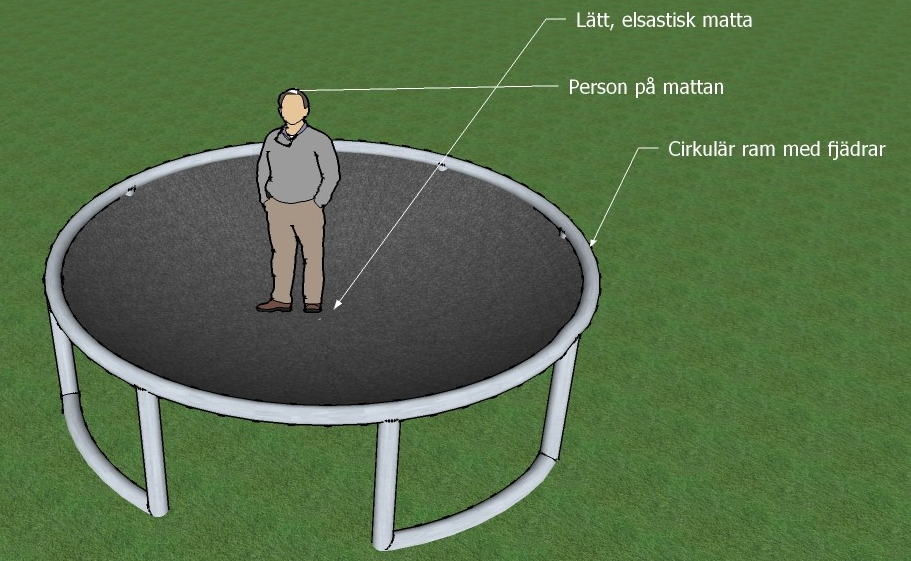
\includegraphics[scale=0.8]{Bild2}
\end{figure}
\clearpage

Figur 1 ger en mycket enkel överblick av vårt system. Studsmattan är helt cirkulär och har fjädrar som sitter radiellt från kanten riktade in mot mitten symmetriskt runt om hela cirkeln. Vi gör antagandet att personen som hoppar står precis i mattans mitt med fötterna tätt ihop.


Insignalen blir i vårt den kraftändring som personen som hoppar utför då denne böjjer eller sträcker på benen. Utsignalen är mattans ändring i höjdled med referenspunkt i jämviktsläget på studsmattan.

Krafterna uttryckta med pilar i bilden är gravitationskraften från massan $F_g$, fjäderns motkraft på massan $F_f$ och kraften från personen som trycker emot $F_a$.

Eftersom fjädrarna är placerade symmetriskt och för att personen står placerad i mitten av mattan kan vi idealisera systemet som en fjäder verkande i y-led eftersom de radiella krafterna tar ut varandra i symmetrin.

\subsection{Gravitationskraften $F_g$}

\begin{equation}
F = m * g * h
\end{equation}

\subsection{Fjäderkraften $F_f$}

(Hookes Lag, k = fjäderkonstant, x = aktuell pos., $x_0$ referens pos.)
\begin{equation}
F = - k * (x - x_0)
\end{equation}

\subsection{Fysik 3}

\subsection{Slutgiltig diff.ekv}

\newpage

\begin{thebibliography}{9}

\bibitem{sune2000}
  Sune Söderkvist,
  \emph{Tidskontinuerliga Signaler \& System}.
  \linebreak
  Erik Larsson AB, Linköping,
  3e upplagan,
  2000.

\end{thebibliography}

\end{document}